\lab{Data Visualization}{Data Visualization}
\label{lab:DataVis}
\objective{
This lab demonstrates how to communicate information through clean, concise, and honest data visualization.
We recommend completing the exercises in a Jupyter Notebook.
}

\section*{The Importance of Visualizations} % =================================

Visualizations of data can reveal insights that are not immediately obvious from simple statistics.
The data set in the following exercise is known as \emph{Anscombe's quartet}.
It is famous for demonstrating the importance of data visualization.

\begin{problem} % Describe Anscombe's Quartet
The file \texttt{anscombe.npy} contains the quartet of data points shown in the table below.
For each section of the quartet,
\begin{itemize}
	\setlength\itemsep{0em}
	\item Plot the data as a scatter plot on the box $[0,20]\times[0,13]$.
    \item Use \li{scipy.stats.linregress()} to calculate the slope and intercept of the least squares regression line for the data and its correlation coefficient (the first three return values).
	\item Plot the least squares regression line over the scatter plot on the domain $x \in [0,20]$.
	\item Report the mean and variance in $x$ and $y$, the slope and intercept of the regression line, and the correlation coefficient.
    Compare these statistics to those of the other sections.
	\item Describe how the section is similar to the others and how it is different.
\end{itemize}
\begin{table}[H]
\scriptsize{
\begin{tabular}{rr|rr|rr|rr}
    \multicolumn{2}{c|}{I}    & \multicolumn{2}{|c|}{II} &
    \multicolumn{2}{|c|}{III} & \multicolumn{2}{|c}{IV} \\
    \multicolumn{1}{c}{$x$}   & \multicolumn{1}{c|}{$y$} &
    \multicolumn{1}{|c}{$x$}  & \multicolumn{1}{c|}{$y$} &
    \multicolumn{1}{|c}{$x$}  & \multicolumn{1}{c|}{$y$} &
    \multicolumn{1}{|c}{$x$}  & \multicolumn{1}{c}{$y$} \\
    \hline
    10.0 & 8.04  & 10.0 & 9.14 & 10.0 & 7.46  & 8.0  & 6.58  \\
    8.0  & 6.95  & 8.0  & 8.14 & 8.0  & 6.77  & 8.0  & 5.76  \\
    13.0 & 7.58  & 13.0 & 8.74 & 13.0 & 12.74 & 8.0  & 7.71  \\
    9.0  & 8.81  & 9.0  & 8.77 & 9.0  & 7.11  & 8.0  & 8.84  \\
    11.0 & 8.33  & 11.0 & 9.26 & 11.0 & 7.81  & 8.0  & 8.47  \\
    14.0 & 9.96  & 14.0 & 8.10 & 14.0 & 8.84  & 8.0  & 7.04  \\
    6.0  & 7.24  & 6.0  & 6.13 & 6.0  & 6.08  & 8.0  & 5.25  \\
    4.0  & 4.26  & 4.0  & 3.10 & 4.0  & 5.39  & 19.0 & 12.50 \\
    12.0 & 10.84 & 12.0 & 9.13 & 12.0 & 8.15  & 8.0  & 5.56  \\
    7.0  & 4.82  & 7.0  & 7.26 & 7.0  & 6.42  & 8.0  & 7.91  \\
    5.0  & 5.68  & 5.0  & 4.74 & 5.0  & 5.73  & 8.0  & 6.89  \\
\end{tabular}}
\end{table}
\label{prob:anscombes-quartet}
\end{problem}

\section*{Improving Specific Types of Visualizations} % =======================

Effective data visualizations show specific comparisons and relationships in the data.
Before designing a visualization, decide what to look for or what needs to be communicated.
Then choose the visual scheme that makes sense for the data.
The following sections demonstrate how to improve commonly used plots to communicate information visually.

\subsection*{Line Plots} % ----------------------------------------------------

\begin{figure}[H] % Horizontal vs. vertical bar chart.
    \centering
    \begin{subfigure}{.47\textwidth}
        \centering
        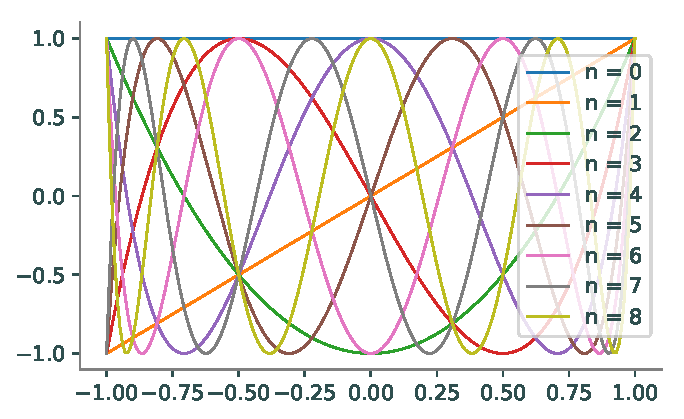
\includegraphics[width=\textwidth]{figures/chebyshev_bad.pdf}
    \end{subfigure}
    %
    \begin{subfigure}{.52\textwidth}
        \centering
        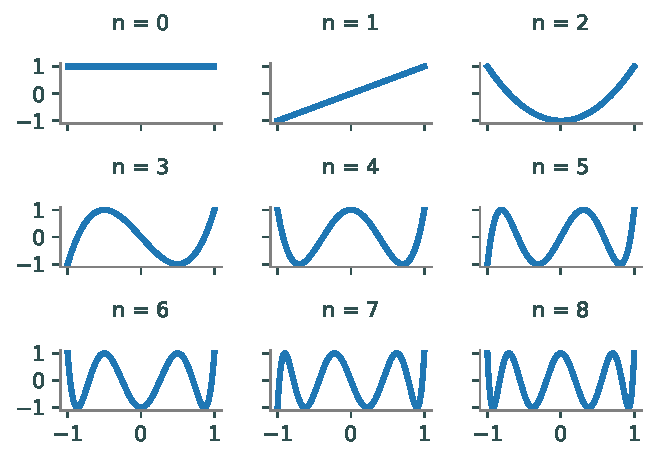
\includegraphics[width=\textwidth]{figures/chebyshev_good.pdf}
    \end{subfigure}
    \caption{Line plots can be used to visualize and compare mathematical functions. For example, this figure shows the first nine Chebyshev polynomials in one plot (left) and small multiples (right). Using small multiples makes comparison easy and shows how each polynomial changes as $n$ increases.}
    \label{fig:chebyshev}
\end{figure}

\begin{lstlisting}
>>> import numpy as np
>>> from matplotlib import pyplot as plt

# Plot the first 9 Chebyshev polynomials in the same plot.
>>> T = np.polynomial.Chebyshev.basis
>>> x = np.linspace(-1, 1, 200)
>>> for n in range(9):
...     plt.plot(x, T(n)(x), label="n = "+str(n))
...
>>> plt.axis([-1.1, 1.1, -1.1, 1.1])        # Set the window limits.
>>> plt.legend(loc="right")
\end{lstlisting}

A line plot connects ordered $(x,y)$ points with straight lines, and is best for visualizing one or two ordered arrays, such as functional outputs over an ordered domain or a sequence of values over time.
Sometimes, plotting multiple lines on the same plot helps the viewer compare two different data sets.
However, plotting several lines on top of each other makes the visualization difficult to read, even with a legend.
For example, Figure \ref{fig:chebyshev} shows the first nine \emph{Chebyshev polynomials}, a family of orthogonal polynomials that satisfies the recursive relation
\[
T_0(x) = 1, \qquad T_1(x) = x, \qquad T_{n+1} = 2xT_n(x) - T_{n-1}(x).
\]
The plot on the right makes comparison easier by using \emph{small multiples}. %, a method made famous by Edward Tufte.
Instead of using a legend, the figure makes a separate subplot with a title for each polynomial.
Adjusting the figure size and the line thickness also makes the information easier to read.

%NumPy's \li{polynomial} module has a convenient tool for constructing these and other important polynomials.%
%\footnote{\li{numpy.polynomial} also has tools for computing other important polynomial families, including the Legendre, Hermite, and Laguerre polynomials.}

\begin{info} % LaTex with Matplotlib text.
Matplotlib titles and annotations can be formatted with \LaTeX, a system for creating technical documents.%
\footnote{See \url{http://www.latex-project.org/} for more information.}
% (this lab manual, for example, is written in \LaTeX).
To do so, use an \li{r} before the string quotation mark and surround the text with dollar signs.
For example, add the following line of code to the loop from the previous example.

\begin{lstlisting}
...     plt.title(r"$T_{}(x)$".<<format>>(n))
\end{lstlisting}

The \li{<<format>>()} method inserts the input $n$ at the curly braces.
The title of the sixth subplot, instead of being ``n = 5,'' will then be ``$T_5(x)$.''
\end{info}

% TODO: Make sure the Bernstein polynomial notation is consistent with the book (it is consistent with Wikipedia currently)

\begin{problem} % Plot the Bernstein polynomials.
The $n+1$ Bernstein basis polynomials of degree $n$ are defined as follows:
\[b_{v,n}(x) = {{n} \choose {v}} x^v (1-x)^{n-v},\qquad v = 0,\ 1,\ \ldots,\ n\]

Plot the first $10$ Bernstein basis polynomials ($n = 0,\ 1,\ 2,\ 3$) as small multiples on the domain $[0,1] \times [0,1]$.
Label the subplots for clarity, adjust tick marks and labels for simplicity, and set the window limits of each plot to be the same.
Consider arranging the subplots so that the rows correspond with $n$ and the columns with $v$.
\\Hint: The constant ${{n} \choose {v}} = \frac{n!}{v!(n-v)!}$ is called the \emph{binomial coefficient} and can be efficiently computed with \li{scipy.special.comb()}.
\end{problem}

\subsection*{Bar Charts} % ----------------------------------------------------

\begin{figure}[H] % Horizontal vs. vertical bar chart.
    \centering
    \begin{subfigure}{.47\textwidth}
        \centering
        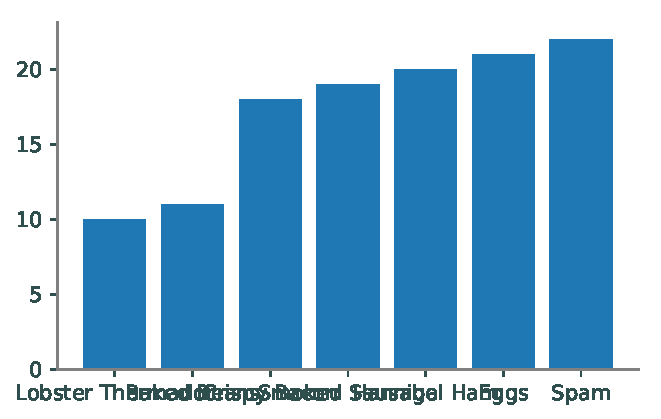
\includegraphics[width=\textwidth]{figures/bar_1.pdf}
    \end{subfigure}
    %
    \begin{subfigure}{.52\textwidth}
        \centering
        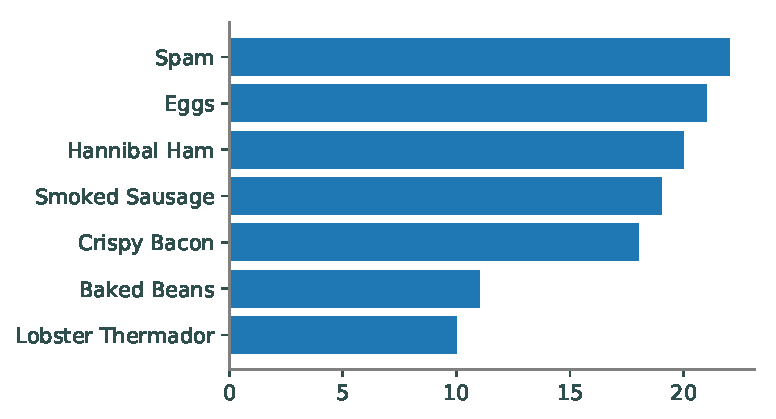
\includegraphics[width=\textwidth]{figures/bar_2.pdf}
    \end{subfigure}
    \caption{Bar charts are used to compare quantities between categorical variables. The labels on the vertical bar chart (left) are more difficult to read than the  labels on the horizontal bar chart (right). Although the labels can be rotated, horizontal text is much easier to read than vertical text.}
\end{figure}

\begin{lstlisting}
>>> labels = ["Lobster Thermador", "Baked Beans", "Crispy Bacon",
...             "Smoked Sausage", "Hannibal Ham", "Eggs", "Spam"]
>>> values = [10, 11, 18, 19, 20, 21, 22]
>>> positions = np.arange(len(labels))

>>> plt.bar(positions, values, align="center")  # Vertical bar chart.
>>> plt.xticks(positions, labels)
>>> plt.show()

>>> plt.barh(positions, values, align="center") # Horizontal bar char (better).
>>> plt.yticks(positions, labels)
>>> plt.tight_layout()
>>> plt.show()
\end{lstlisting}

A bar chart plots categorical data in a sequence of bars.
They are best for small, discrete, one-dimensional data sets.
In Matplotlib, \li{plt.bar()} creates a vertical bar chart or \li{plt.barh()} creates a horizontal bar chart.
These functions receive the locations of each bar followed by the height of each bar (as lists or arrays).
In most situations, horizontal bar charts are preferable to vertical bar charts because horizontal labels are easier to read than vertical labels.
Data in a bar chart should also be sorted in a logical way, such as alphabetically, by size, or by importance.

\subsection*{Histograms} % ----------------------------------------------------

\begin{figure}[H] % Cleaning up a histogram.
    \centering
    \begin{subfigure}{.47\textwidth}
        \centering
        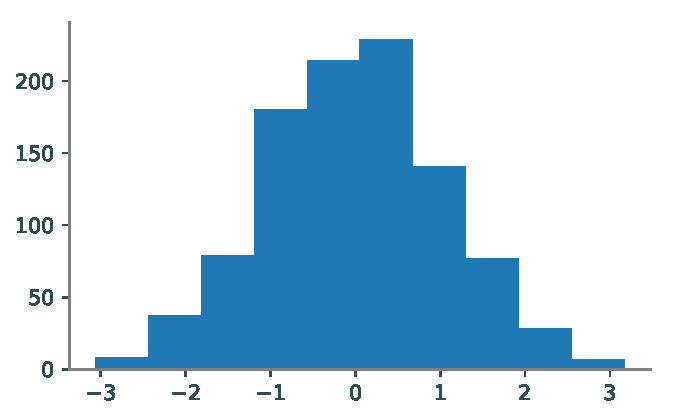
\includegraphics[width=\textwidth]{figures/hist1.pdf}
    \end{subfigure}
    %
    \begin{subfigure}{.47\textwidth}
        \centering
        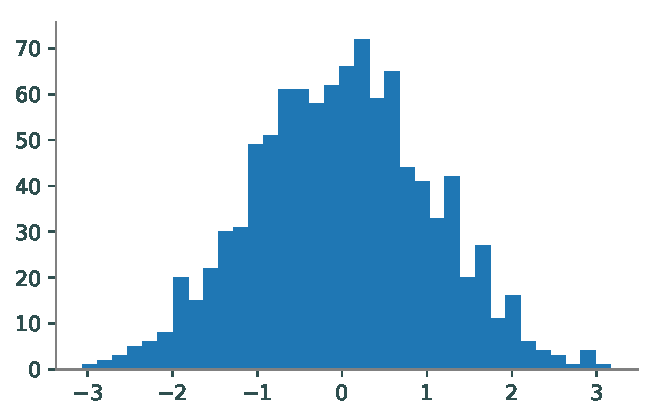
\includegraphics[width=\textwidth]{figures/hist2.pdf}
    \end{subfigure}
    \caption{Histograms are used to show the distribution of one-dimensional data. Experimenting with different values for the bin size is important when plotting a histogram. Using only 10 bins (left) doesn't give a good sense for how the randomly generated data is distributed. However, using 35 bins (right) reveals the shape of a normal distribution.}
\end{figure}

\begin{lstlisting}
>>> data = np.random.normal(size=10000)
>>> fig, ax = plt.subplots(1, 2)
>>> ax[0].hist(data, bins=10)
>>> ax[1].hist(data, bins=35)
\end{lstlisting}

A histogram partitions an interval into a number of bins and counts the number of values that fall into each bin.
Histograms are ideal for visualizing how unordered data in a single array is distributed over an interval.
For example, if data are drawn from a probability distribution, a histogram approximates the distribution's probability density function.
Use \li{plt.hist()} to create a histogram.
The arguments \li{bins} and \li{<<range>>} specify the number of bins to draw and over what domain.
A histogram with too few or too many bins will not give a clear view of the distribution.

\subsection*{Scatter Plots} % -------------------------------------------------

\begin{figure}[H] % Heat maps and contour plots.
    \centering
    \begin{subfigure}{.47\textwidth}
        \centering
        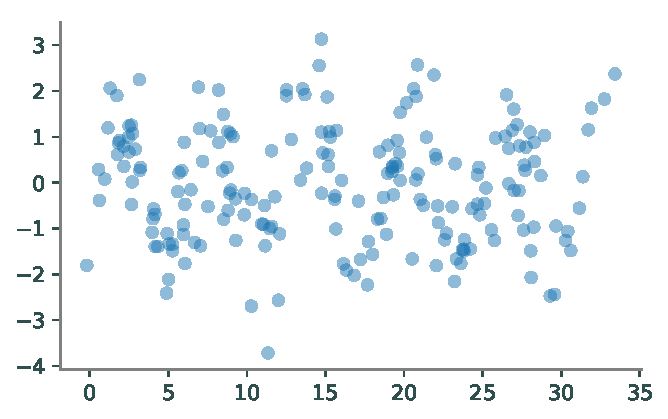
\includegraphics[width=\textwidth]{figures/alpha1.pdf}
    \end{subfigure}
    %
    \begin{subfigure}{.47\textwidth}
        \centering
        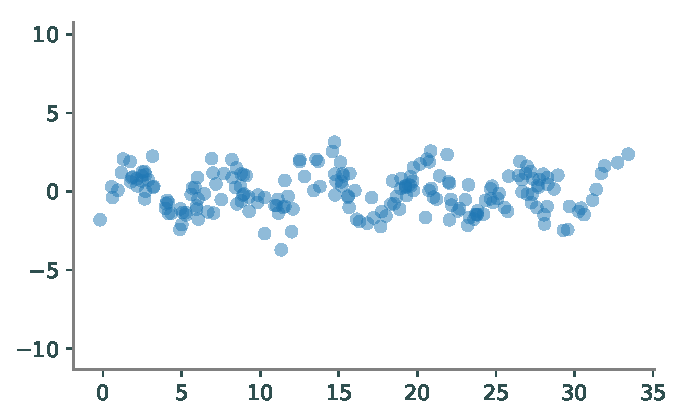
\includegraphics[width=\textwidth]{figures/alpha2.pdf}
    \end{subfigure}
    \caption{Scatter plots show correlation between variables by plotting markers at coordinate points. The figure above displays randomly perturbed data visualized using two scatter plots with \li{alpha=.5} and \li{edgecolor='none'}. The default (left) makes it harder to see correlation and pattern whereas making the axes equal better reveals the oscillatory behavior in the perturbed sine wave.}
    \label{fig:scatter_scales}
\end{figure}

\begin{lstlisting}
>>> np.random.seed(0)
>>> x = np.linspace(0,10*np.pi,200) + np.random.normal(size=200)
>>> y = np.sin(x) + np.random.normal(size=200)

>>> plt.scatter(x, y, alpha=.5, edgecolor='none')
>>> plt.show()

>>> plt.scatter(x, y, alpha=.5, edgecolor='none')
>>> plt.axis('equal')
>>> plt.show()
\end{lstlisting}

A scatter plot draws $(x,y)$ points without connecting them.
Scatter plots are best for displaying data sets without a natural order, or where each point is a distinct, individual instance.
They are frequently used to show correlation between variables in a data set.
Use \li{plt.scatter()} to create a scatter plot.%
\footnote{Scatter plots can also be drawn with with \lif{plt.plot()} by specifying a point marker such as \lif{'.'}, \lif{','}, \lif{'o'}, or \lif{'+'}.
The keywords \lif{s} and \lif{c} can be used to change the marker size and marker color, respectively.}

Similar data points in a scatter plot may overlap, as in Figure \ref{fig:scatter_scales}.
Specifying an \emph{alpha value} reveals overlapping data by making the markers transparent (see Figure \ref{fig:scatter_hexbin} for an example).
The keyword \li{alpha} accepts values between 0 (completely transparent) and 1 (completely opaque).
When plotting lots of overlapping points, the outlines on the markers can make the visualization look cluttered.
Setting the edgecolor keyword to zero removes the outline and improves the visualization.

\begin{problem} % Scatter plots with visualizations.
The file \texttt{MLB.npy} contains measurements from over 1,000 recent Major League Baseball players, compiled by UCLA.\footnote{See \url{http://wiki.stat.ucla.edu/socr/index.php/SOCR_Data_MLB_HeightsWeights}.}
Each row in the array represents a player; the columns are the player's height (in inches), weight (in pounds), and age (in years), in that order.

Create several visualizations to show the correlations between height, weight, and age in the MLB data set.
Use at least one scatter plot.
Adjust the marker size, plot a regression line, change the window limits, and use small multiples where appropriate.
\end{problem}

\begin{problem} % Earthquake data
The file \texttt{earthquakes.npy} contains data from over 17,000 earthquakes between 2000 and 2010 that were at least a 5 on the Richter scale.%
\footnote{See \url{http://earthquake.usgs.gov/earthquakes/search/}.}
Each row in the array represents an earthquake;
the columns are the earthquake's date (as a fraction of the year), magnitude (on the Richter scale), longitude, and latitude, in that order.

Because each earthquake is a distinct event, a good way to start visualizing this data might be a scatter plot of the years versus the magnitudes of each earthquake.

\begin{lstlisting}
>>> year, magnitude, longitude, latitude = np.load("earthquakes.npy").T
>>> plt.plot(year, magnitude, '.')
>>> plt.xlabel("Year")
>>> plt.ylabel("Magnitude")
\end{lstlisting}

\begin{figure}[H] % Bad visualization: earthquake data, year vs magnitude.
    \centering
    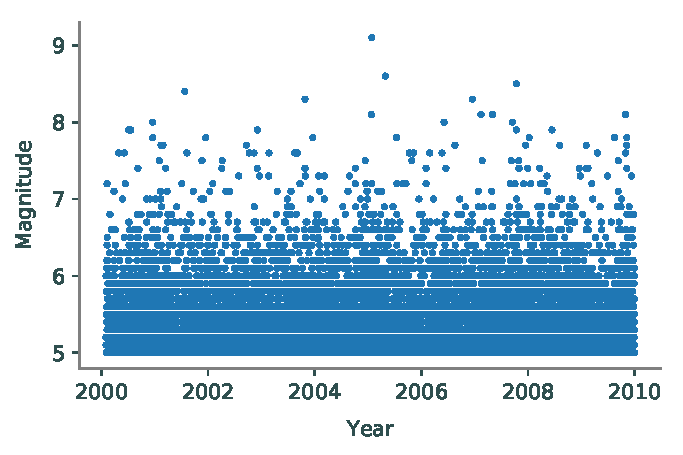
\includegraphics[width=.7\textwidth]{figures/earthquake.pdf}
\end{figure}

Unfortunately, this plot communicates very little information because the data is so cluttered.
Describe the data with at least two better visualizations, including line plots, scatter plots, and histograms as appropriate.
Your plots should answer the following questions:
\begin{enumerate}
    \item How many earthquakes happened every year?
    \item How often do stronger earthquakes happen compared to weaker ones?
    \item Where do earthquakes happen? Where do the strongest earthquakes happen?
    \\(Hint: Use \li{plt.axis("equal")} or \li{ax.set_aspect("equal")} to fix the aspect ratio, which may improve comparisons between longitude and latitude.)
\end{enumerate}
\end{problem}

\subsection*{Hexbins} % -------------------------------------------------------

\begin{figure}[H] % Hexbins
    \centering
    \begin{subfigure}{.47\textwidth}
        \centering
        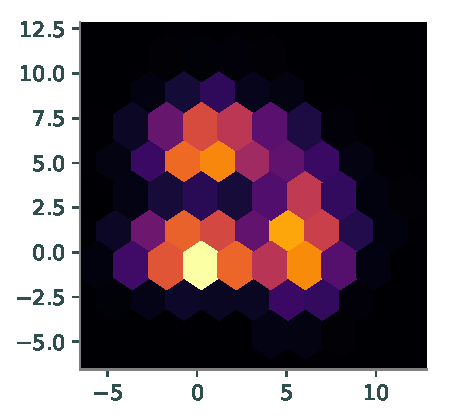
\includegraphics[width=\textwidth]{figures/hexbin_1.pdf}
    \end{subfigure}
    %
    \begin{subfigure}{.47\textwidth}
        \centering
        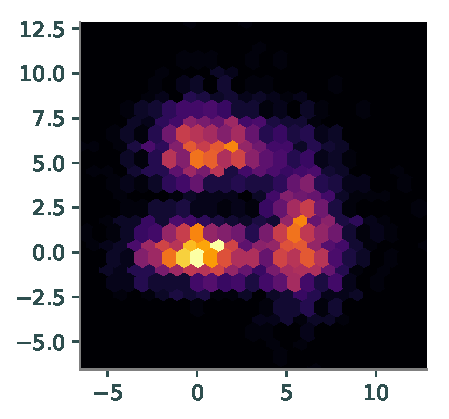
\includegraphics[width=\textwidth]{figures/hexbin_2.pdf}
    \end{subfigure}
    %
    \caption{Hexbins can be used instead of using a three-dimensional histogram to show the distribution of two-dimensional data. Choosing the right gridsize will give a better picture of the distribution. The figure above shows random data plotted as hexbins with a gridsize of 10 (left) and 25 (right). Hexbins use color to show height via a colormap and both histograms above use the \li{'inferno'} colormap.}
    \label{fig:scatter_hexbin}
\end{figure}

\begin{lstlisting}
# Add random draws from various distributions in two dimensions.
>>> a = np.random.exponential(size=1000) + np.random.normal(size=1000) + 5
>>> b = np.random.exponential(size=1000) + 2*np.random.normal(size=1000)
>>> x = np.hstack((a, b, 2*np.random.normal(size=1000)))
>>> y = np.hstack((b, a,   np.random.normal(size=1000)))

# Plot the samples with hexbins of gridsize 10 and 25.
>>> fig, axes = plt.subplots(1, 2)
>>> window = [x.min(), x.max(), y.min(), y.max()]
>>> for ax, size in zip(axes, [10, 25]):
...     ax.hexbin(x, y, gridsize=size, cmap='inferno')
...     ax.axis(window)
...     ax.set_aspect("equal")
...
>>> plt.show()
\end{lstlisting}

A \emph{hexbin} is a way of representing the frequency of ocurrances in a two-dimensional plane.
Similar to a histogram, which sorts one-dimensional data into bins, a hexbin sorts two-dimensional data into hexagonal bins arranged in a grid and uses color instead of height to show frequency.
Creating an effective hexbin relies on choosing an appropriate \li{gridsize} and colormap.
The \emph{colormap} is a function that assigns data points to an ordering of colors.
Use \li{plt.hexbin()} to create a hexbin and use the \li{cmap} keyword to specify the colormap.

\subsection*{Heat Maps and Contour Plots} % -----------------------------------

\begin{figure}[H] % Heat maps and contour plots.
    \centering
    \begin{subfigure}{.495\textwidth}
        \centering
        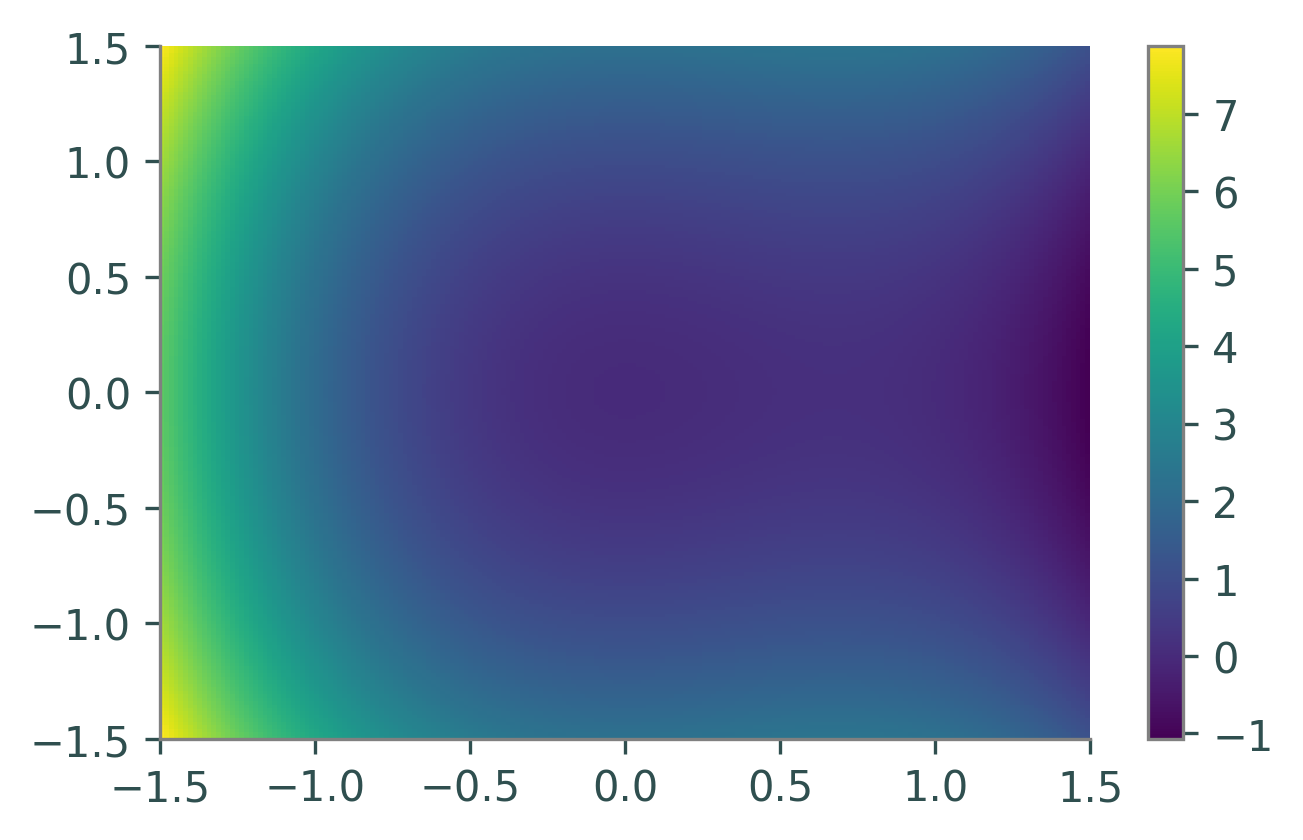
\includegraphics[width=\textwidth]{figures/heatmap_1.png}
    \end{subfigure}
    %
    \begin{subfigure}{.495\textwidth}
        \centering
        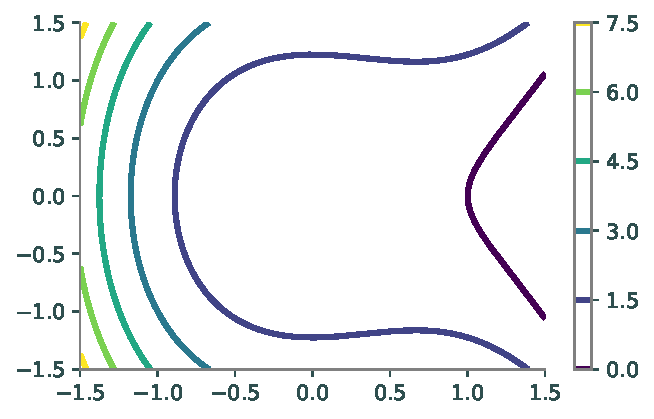
\includegraphics[width=\textwidth]{figures/contour_1.pdf}
    \end{subfigure}
    \\
    \begin{subfigure}{.495\textwidth}
        \centering
        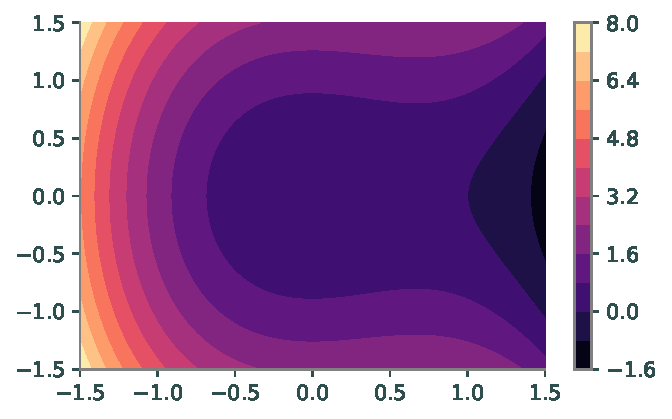
\includegraphics[width=\textwidth]{figures/contour_2.pdf}
    \end{subfigure}
    %
    \begin{subfigure}{.495\textwidth}
        \centering
        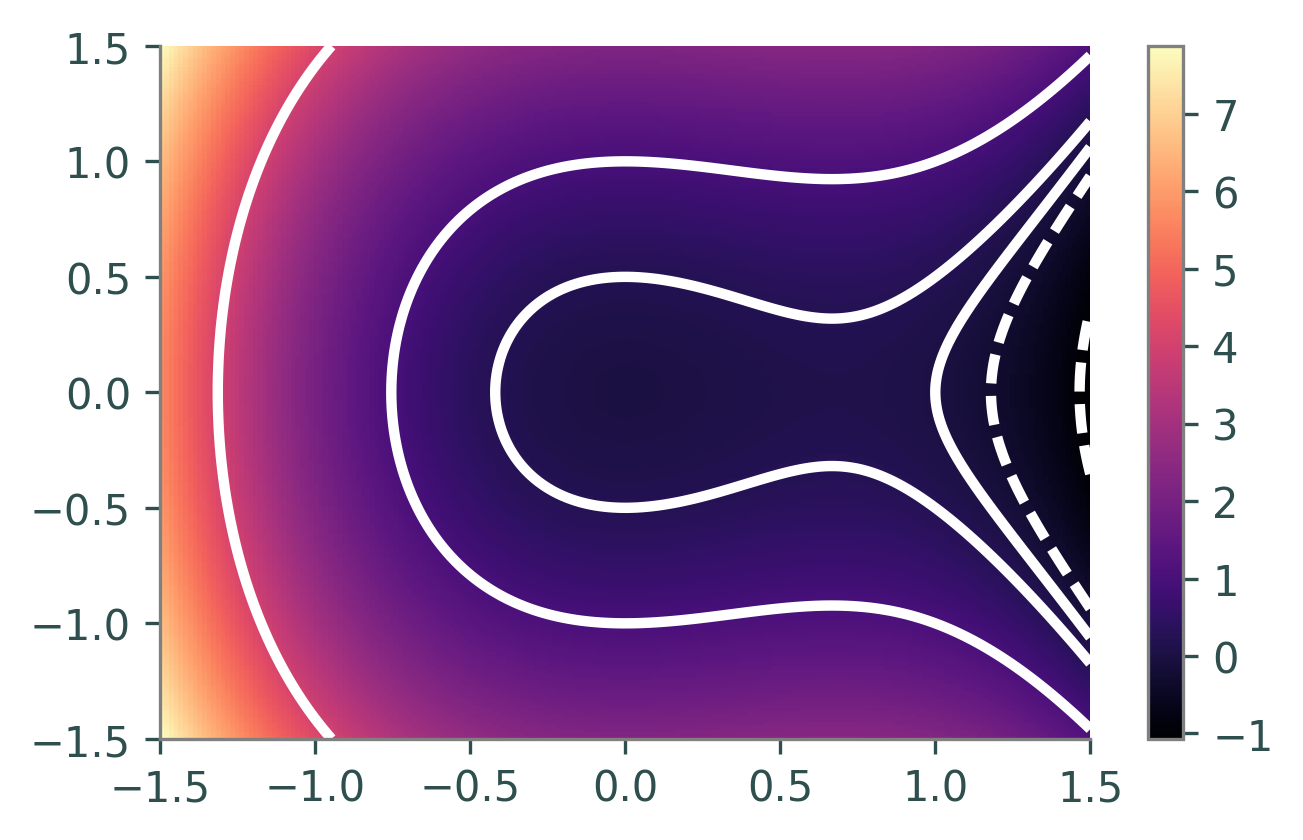
\includegraphics[width=\textwidth]{figures/heatmap_2.png}
    \end{subfigure}
    \caption{Heat maps visualize three-dimensional functions or surfaces by using color to represent the value in one dimension. With continuous data, it can be hard to identify regions of interest. Contour plots solve this problem by visualizing the level curves of the surface. Top left: heat map. Top right: contour plot. Bottom left: heat map. Bottom right: contours plotted on a heat map.}
    \label{fig:heatcontour}
\end{figure}

\begin{lstlisting}
# Construct a 2-D domain with np.meshgrid() and calculate f on the domain.
>>> x = np.linspace(-1.5, 1.5, 200)
>>> X, Y = np.meshgrid(x, x)
>>> Z = Y**2 - X**3 + X**2

# Plot f using a heat map, a contour map, and a filled contour map.
>>> fig, ax = plt.subplots(2,2)
>>> ax[0,0].pcolormesh(X, Y, Z, cmap="viridis")     # Heat map.
>>> ax[0,1].contour(X, Y, Z, 6, cmap="viridis")     # Contour map.
>>> ax[1,0].contourf(X, Y, Z, 12, cmap="magma")   # Filled contour map.


# Plot specific level curves and a heat map with a colorbar.
>>> ax[1,1].contour(X, Y, Z, [-1, -.25, 0, .25, 1, 4], colors="white")
>>> cax = ax[1,1].pcolormesh(X, Y, Z, cmap="magma")
>>> fig.colorbar(cax, ax=ax[1,1])

>>> plt.show()
\end{lstlisting}

Let $f:\mathbb{R}^2\rightarrow\mathbb{R}$ be a scalar-valued function on a 2-dimensional domain.
A \emph{heat map} of $f$ assigns a color to each $(x,y)$ point in the domain based on the value of $f(x,y)$, while a contour plot is a drawing of the \emph{level curves} of $f$.
The level curve corresponding to the constant $c$ is the set $\left\{(x,y)\mid c = f(x,y)\right\}$.
A filled contour plot colors in the sections between the level curves and is a discretized version of a heat map.
The values of $c$ corresponding to the level curves are automatically chosen to be evenly spaced over the range of values of $f$ on the domain.
However, it is sometimes better to strategically specify the curves by providing a list of $c$ constants.

Consider the function $f(x,y) = y^2 - x^3 + x^2$ on the domain $[-\frac{3}{2}, \frac{3}{2}] \times [-\frac{3}{2}, \frac{3}{2}]$.
A heat map of $f$ reveals that it has a large basin around the origin.
Since $f(0,0) = 0$, choosing several level curves close to $0$ more closely describes the topography of the basin.
The fourth subplot in \ref{fig:heatcontour} uses the curves with $c = -1,\ -\frac{1}{4},\ 0,\ \frac{1}{4},\ 1,$ and $4$.

When plotting hexbins, heat maps, and contour plots, be sure to choose a colormap that best represents the data.
Avoid using spectral or rainbow colormaps like \li{"jet"} because they are not \emph{perceptually uniform}, meaning that the rate of change in color is not constant.
Because of this, data points may appear to be closer together or farther apart than they actually are.
This creates visual false positives or false negatives in the visualization and can affect the interpretation of the data.
As a default, we recommend using the sequential colormaps \li{"viridis"} or \li{"inferno"} because they are designed to be perceptually uniform and colorblind friendly.
For the complete list of Matplotlib color maps, see \url{http://matplotlib.org/examples/color/colormaps_reference.html}.

\begin{problem} % Rosenbrock
The \emph{Rosenbrock function} is defined as
\[f(x,y) = (1-x)^2 + 100(y-x^2)^2.\]
The minimum value of $f$ is $0$, which occurs at the point $(1,1)$ at the bottom of a steep, banana-shaped valley of the function.

Use a heat map and a contour plot to visualize the Rosenbrock function.
Also plot the minimizer $(1,1)$.
Use a different sequential colormap for each visualization.
\end{problem}

\section*{Best Practices} % ===============================================

Good scientific visualizations make comparison easy and clear.
The eye is very good at detecting variation in one dimension and poor in two or more dimensions.
For example, consider Figure \ref{fig:piebar}.
Despite the difficulty, most people can probably guess which slice of a pie chart is the largest or smallest.
However, it's almost impossible to confidently answer the question \emph{by how much?} The bar charts may not be as aesthetically pleasing but they make it much easier to precisely compare the data.
Avoid using pie charts as well as other visualizations that make accurate comparison difficult, such as radar charts, bubble charts, and stacked bar charts.

\begin{figure}[H] % Pie chart --> Bar chart
    \centering
    \begin{subfigure}{.49\textwidth}
        \centering
        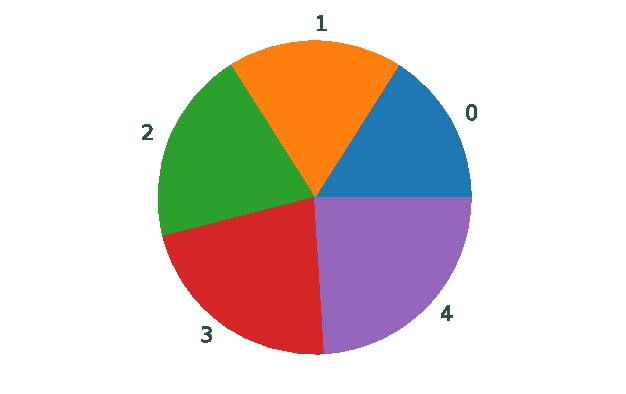
\includegraphics[width=\textwidth]{figures/piechart1.pdf}
    \end{subfigure}
    %
    \begin{subfigure}{.49\textwidth}
        \centering
        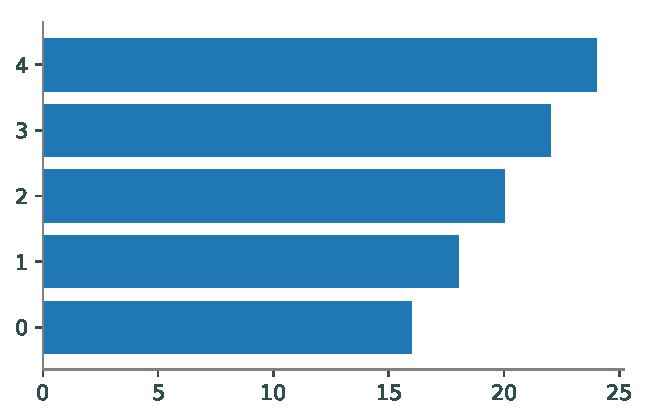
\includegraphics[width=\textwidth]{figures/piebar1.pdf}
    \end{subfigure}
    %
    \begin{subfigure}{.49\textwidth}
        \centering
        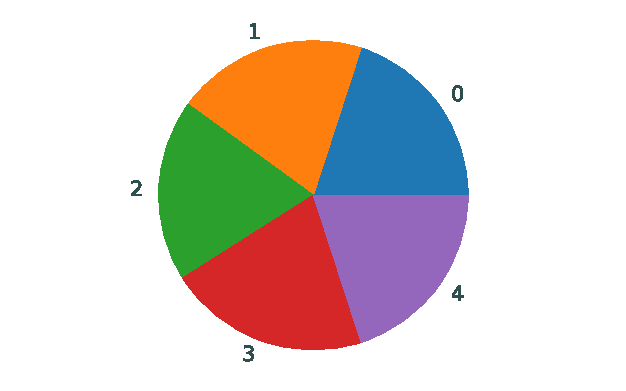
\includegraphics[width=\textwidth]{figures/piechart2.pdf}
    \end{subfigure}
    %
    \begin{subfigure}{.49\textwidth}
        \centering
        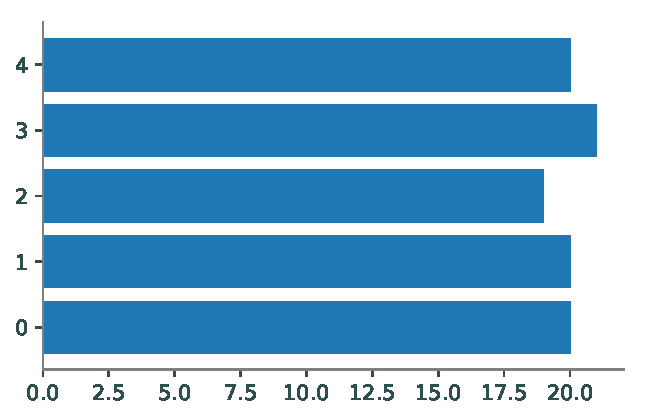
\includegraphics[width=\textwidth]{figures/piebar2.pdf}
    \end{subfigure}
    %
    \begin{subfigure}{.49\textwidth}
        \centering
        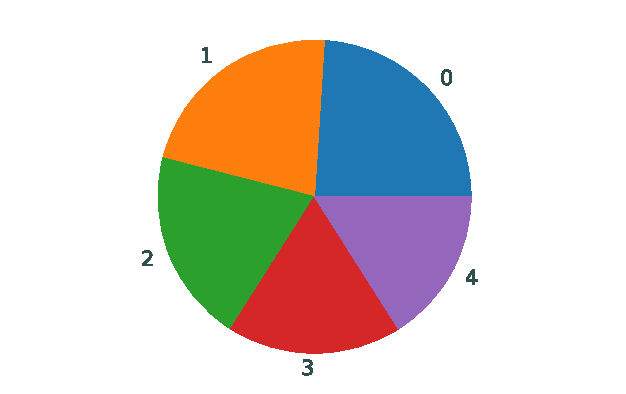
\includegraphics[width=\textwidth]{figures/piechart3.pdf}
    \end{subfigure}
    \begin{subfigure}{.49\textwidth}
        \centering
        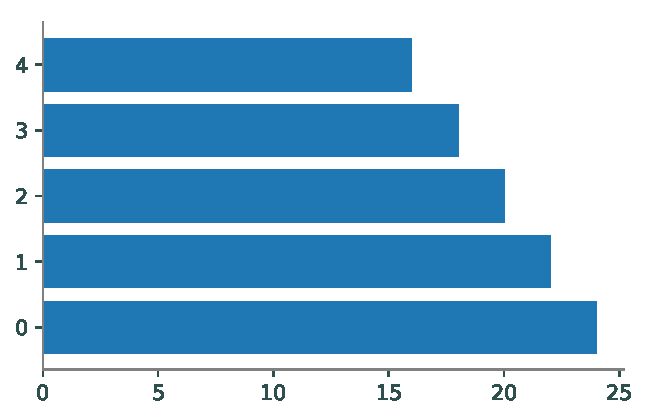
\includegraphics[width=\textwidth]{figures/piebar3.pdf}
    \end{subfigure}
    %
    \caption{The pie charts on the left may be more colorful but it's extremely difficult to quantify the difference between each slice. Instead, the horizontal bar charts on the right make it very easy to see the difference between each variable.}
    \label{fig:piebar}
\end{figure}

No visualization perfectly represents data, but some are better than others.
Finding the best visualization for a data set is an iterative process.
Experiment with different visualizations by adjusting their parameters: color, scale, size, shape, position, and length.
It may be necessary to use a data transformation or visualize various subsets of the data.
As you iterate, keep in mind the saying attributed to George Box: ``All models are wrong, but some are useful.''
Do whatever is needed to make the visualization useful and effective.

\begin{figure}[H] % BAR CHART MONSTROSITY!
    \centering
    \begin{subfigure}{.47\textwidth}
        \centering
        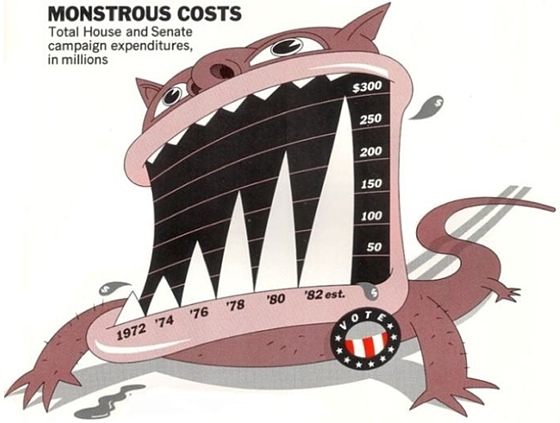
\includegraphics[width=\textwidth]{figures/chartjunk1.jpg}
    \end{subfigure}
    %
    \begin{subfigure}{.47\textwidth}
        \centering
        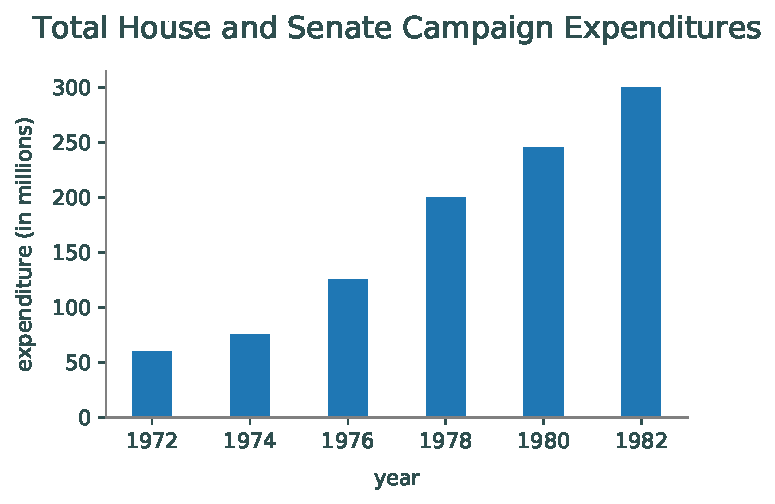
\includegraphics[width=\textwidth]{figures/chartjunk_improved.pdf}
    \end{subfigure}
    \caption{Chartjunk refers to anything that does not communicate data. In the image on the left, the cartoon monster distorts the bar chart and manipulates the feelings of the viewer to think negatively about the results. The image on the right shows the same data without chartjunk, making it simple and very easy to interpret the data objectively.}
    \label{fig:chartjunk}
\end{figure}

Good visualizations are as simple as possible and no simpler.
Edward Tufte coined the term \emph{chartjunk} to mean anything (pictures, icons, colors, and text) that does not represent data or is distracting.
Though chartjunk might appear to make data graphics more memorable than plain visualizations, \textbf{it is more important to be clear and precise in order to prevent misinterpretation}.
The physicist Richard Feynman said, ``For a successful technology, reality must take precedence over public relations, for Nature cannot be fooled.'' Remove chartjunk and anything that prevents the viewer from objectively interpreting the data.

\begin{figure}[H] % Heat maps and contour plots.
    \centering
    \begin{subfigure}{.495\textwidth}
        \centering
        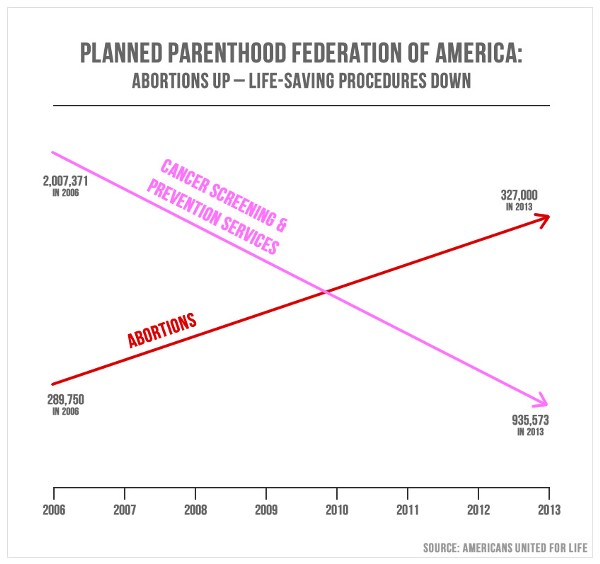
\includegraphics[width=\textwidth]{figures/plannedparenthood}
    \end{subfigure}
    %
    \begin{subfigure}{.495\textwidth}
        \centering
        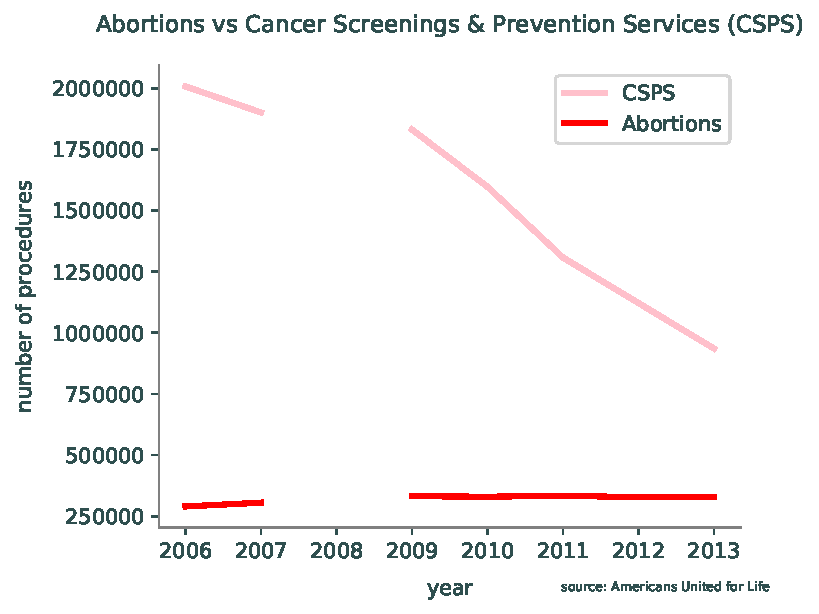
\includegraphics[width=\textwidth]{figures/planparent_corrected}
    \end{subfigure}
    \caption{The chart on the left is an example of a dishonest graphic shown at a United States congressional hearing in 2015. The chart on the right shows a more accurate representation of the data by showing the y-axis and revealing the missing data from 2008. Source: PolitiFact.}
    \label{fig:planparent}
\end{figure}

Visualizations should be honest.
Figure \ref{fig:planparent} shows how visualizations can be dishonest.
The misleading graphic on the left was used as evidence in a United States congressional hearing in 2015.
With the $y$-axis completely removed, it is easy to miss that each line is shown on a different $y$-axis even though they are measured in the same units.
Furthermore, the chart fails to indicate that data is missing from the year 2008.
The graphic on the right shows a more accurate representation of the data.\footnote{For more information about this graphic, visit \url{http://www.politifact.com/truth-o-meter/statements/2015/oct/01/jason-chaffetz/chart-shown-planned-parenthood-hearing-misleading-/}.}

Never use data visualizations to deceive or manipulate.
Always present information on who created it, where the data came from, how it was collected, whether it was cleaned or transformed, and whether there are conflicts of interest or possible biases present.
Use specific titles and axis labels, and include units of measure.
Choose an appropriate window size and use a legend or other annotations where appropriate.

\begin{problem}
The file \texttt{countries.npy} contains information from 20 different countries.
Each row in the array represents a different country; the columns are the 2015 population (in millions of people), the 2015 GDP (in billions of US dollars), the average male height (in centimeters), and the average female height (in centimeters), in that order.%
\footnote{
See \url{https://en.wikipedia.org/wiki/List_of_countries_by_GDP_(nominal)},
\\ \url{https://en.wikipedia.org/wiki/List_of_countries_and_dependencies_by_population}, and
\\ \url{http://www.averageheight.co/}.
}

The countries corresponding are listed below in order.

\begin{lstlisting}
countries = ["Austria", "Bolivia", "Brazil", "China",
            "Finland", "Germany", "Hungary", "India",
            "Japan", "North Korea", "Montenegro", "Norway",
            "Peru", "South Korea", "Sri Lanka", "Switzerland",
            "Turkey", "United Kingdom", "United States", "Vietnam"]
\end{lstlisting}

Visualize this data set with at least four plots, using at least one scatter plot, one histogram, and one bar chart.
List the major insights that your visualizations reveal.
\\(Hint: consider using \li{np.argsort()} and fancy indexing to sort the data for the bar chart.)
\end{problem}

For more about data visualization, we recommend the following books and websites.
\begin{itemize}
    \item \emph{How to Lie with Statistics} by Darrell Huff (1954).
    \item \emph{The Visual Display of Quantitative Information} by Edward Tufte (2nd edition).
    \item \emph{Visual Explanations} by Edward Tufte.
    \item \emph{Envisioning Information} by Edward Tufte.
    \item \emph{Beautiful Evidence} by Edward Tufte.
    \item \emph{The Functional Art} by Alberto Cairo.
    \item \emph{Visualization Analysis and Design} by Tamara Munzner.
    \item \emph{Designing New Default Colormaps}: \url{https://bids.github.io/colormap/}.
\end{itemize}
